\section{Design pattern}

Un \glossario{Design Pattern} descrive problemi che si ripetono molteplici volte nel nostro ambiente. Oltre al problema descrive anche soluzioni eleganti ad esso e i risultati che si ottengono nell'applicarlo. È fondamentale per qualsiasi progettista conoscere a fondo i \glossario{Design Pattern}, in quanto facilita l'attività di progettazione, favorisce la riusabilità e dà benefici enormi in termini di manutenibilità. Fondamentalmente possiamo suddividere i \glossario{Design Pattern} in quattro categorie:

\begin{itemize}

	\item \textbf{\glossario{Design Pattern} architetturali}, che esprimono schemi di base per impostare l'organizzazione strutturale di un sistema software;
	\item \textbf{\glossario{Design Pattern} creazionali}, che forniscono un'astrazione del processo di istanziazione degli oggetti;
	\item \textbf{\glossario{Design Pattern} strutturali}, che si occupano delle modalità di composizione di classi e oggetti per formare strutture complesse; 
	\item \textbf{\glossario{Design Pattern} comportamentali}, che si occupano di algoritmi e dell'assegnamento di responsabilità tra oggetti collaboranti.

\end{itemize}

Per un approfondimento e un richiamo teorico dei \glossario{Design Pattern} utilizzati nel progetto \glossario{MaaP} si rimanda all'Appendice \ref{appendice-pattern}. In seguito verranno descritti i \glossario{Design Pattern} implementati.

\textit{Nota: alcune immagini del presente capitolo non sono UML standard ma si sono semplici ritagli di diagrammi già presenti e visualizzati nei capitoli precedenti. Questo è stato fatto per fornire una visualizzazione mirata del contesto in cui viene utilizzato il design pattern.}

\subsection{Design Pattern Architetturali}

\subsubsection{MVC}

\begin{itemize}

	\item \textbf{Scopo}: Questo pattern è utilizzato per separare le responsabilità dell'applicazione a diversi componenti e permettere di fare una chiara divisione presentazione, struttura dei dati e operazioni su di essi.
	\item \textbf{Utilizzo}: Viene utilizzato dall'applicazione principalmente per delegare il ruolo di presentazione dei dati al \glossario{front-end}, lasciando al \glossario{back-end} la gestione della logica dell'applicazione (autenticazione, corrispondenza tra \glossario{API} e operazioni sui dati) e la logica di business. Nel \glossario{back-end} è presente una chiara distinzione tra questi tre componenti:
	\begin{itemize}
		\item Il package \texttt{Back-end::Lib::Model} è la componente \textbf{model} del pattern, e si occupa di gestire la logica interna dei dati degli utenti e delle \glossario{Collections}. Costruisce dei modelli di dati interfacciandosi con il database \glossario{MongoDB};
		\item Il package \texttt{Back-end::Lib::View} è la componente \textbf{view} del pattern, e si occupa di fornire un template per la composizione delle email da inviare per il recupero della password. Le richieste inoltrate al \glossario{back-end}, inoltre, ricevono come risposta dei dati in formato \glossario{JSON}. La rappresentazione dei dati che viene fornita in output può essere considerata implicitamente la componente \textbf{view} dell'intero package;
		\item Il package \texttt{Back-end::Lib::Controller} è la componente \textbf{controller} del pattern, e si occupa ricevere le richieste in ingresso, di interagire quindi con il \textit{model} prelevando i dati e di restituirli al richiedente in formato \glossario{JSON}.
	\end{itemize}
	
\end{itemize}

\begin{figure}[H]
\centering 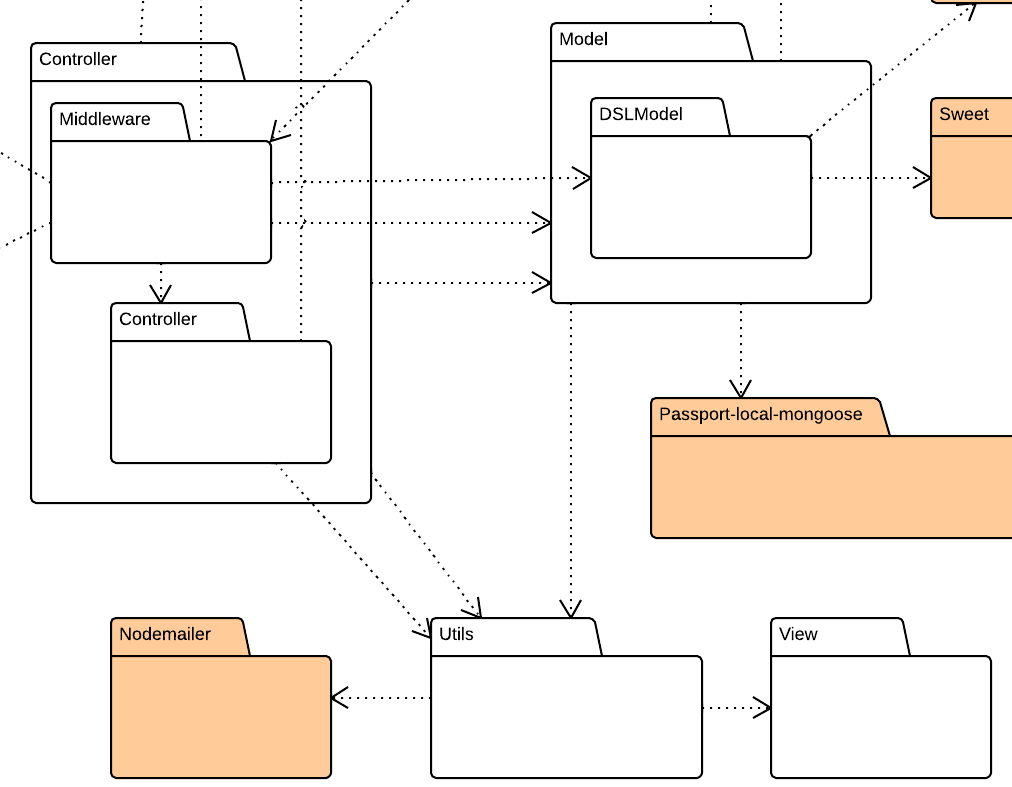
\includegraphics[width=0.6\textwidth]{patterns/contestualizzazione/mvc.png}
\caption{Contestualizzazione di MVC}
\label{fig:mvc}
\end{figure}

\subsubsection{MVW}

\begin{itemize}

	\item \textbf{Scopo}: È un \glossario{Design Pattern} simile a \glossario{MVC} che permette di avere una corrispondenza più diretta e automatica tra la \textit{view} e il \textit{model}. L'acronimo \glossario{MVW} sta per \textit{Model-View-Whatever}, dove \textit{Whatever}, secondo i progettisti di \glossario{Angular.js}, indica "\textit{whatever works for you}".
	\item \textbf{Utilizzo}: È il \glossario{Design Pattern} utilizzato dal \glossario{framework} \glossario{Angular.js}, con il quale viene sviluppata la parte \glossario{front-end} dell'applicazione \glossario{MaaP}. Un maggiore approfondimento è fornito in appendice.

\end{itemize}

\subsubsection{Middleware} 

\begin{itemize}

	\item \textbf{Scopo}: Si è scelto di utilizzare questo \glossario{Design Pattern} per fornire un \textit{intermediario} tra i vari componenti software dell'applicazione in modo da semplificare notevolmente la loro connessione e collaborazione. Questo pattern in generale è molto utile nello sviluppo e nella gestione di di sistemi distribuiti complessi, e in questo contesto il progetto \glossario{MaaP} si colloca perfettamente.
	\item \textbf{Utilizzo}: Viene utilizzato dal \glossario{framework} \glossario{Express} attraverso il modulo \textit{connect} per fornire una libreria di funzioni comuni. Definisce una serie di \textit{livelli} (o funzioni) per gestire le varie richieste dell'applicazione e richiamare i rispettivi \textit{handler}. Tutti i componenti del middleware sono collegati l'uno con l'altro e ricevono a turno una richiesta in ingresso, finché uno di questi non decide di partire con l'elaborazione per poi chiamare la funzione \texttt{next}. Come si può notare è molto legato a \glossario{Chain of Responsibility}, che verrà descritto in seguito. Tutti i componenti di \glossario{Express} vengono utilizzati con il metodo \texttt{use} di \glossario{Express}. Nella progettazione architetturale è utilizzato nel package \texttt{Back-End::Lib::Middleware}.

\end{itemize}

\begin{figure}[H]

\centering 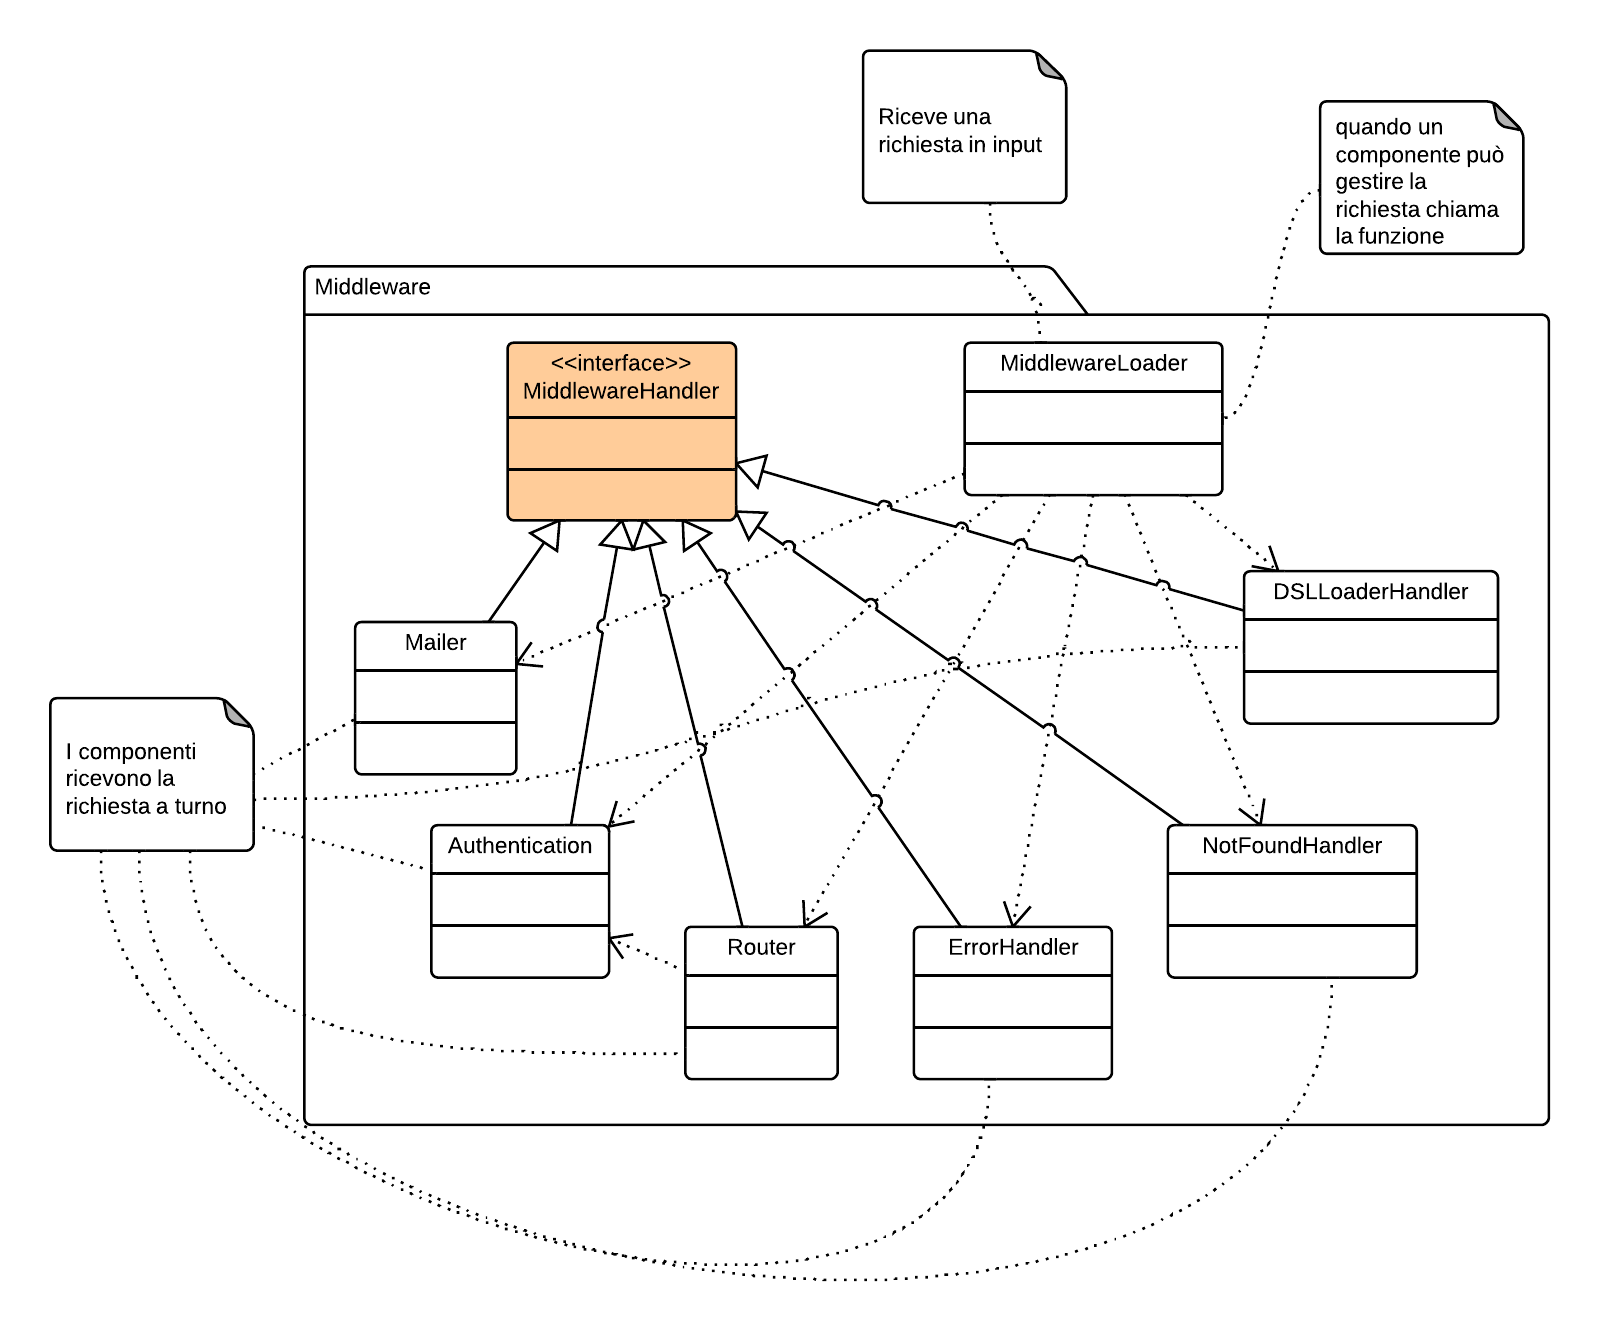
\includegraphics[width=0.8\textwidth]{patterns/contestualizzazione/middleware.png}
\caption{Contestualizzazione di Middleware}
\label{fig:mvc}
\end{figure}

\subsection{Design Pattern Creazionali}

\subsubsection{Registry}

\begin{itemize}

	\item \textbf{Scopo}: Viene utilizzato per ottenere oggetti a partire da altri oggetti che hanno un'associazione con esso. Questa ricerca viene effettuata tramite una \textit{classe registro}, che conterrà una funzione di ricerca in base a una chiave.
	\item \textbf{Utilizzo}: Le diverse \glossario{Collection} presenti nell'applicazione si differenziano per il loro nome. Utilizzando questo pattern, quando arriva una richiesta la classe che lo implementa sarà in grado di fornire il file \glossario{DSL} corretto in quanto possiederà al suo interno un registro sul quale sarà possibile effettuare una ricerca. È implementato nella classe \texttt{Back-End::Lib::DSLModel}. Alla sua creazione verrà caricato il registro. Questa classe inoltre conterrà un metodo di ricerca e un metodo di caricamento del file DSL.

\end{itemize}

\begin{figure}[H]

\centering 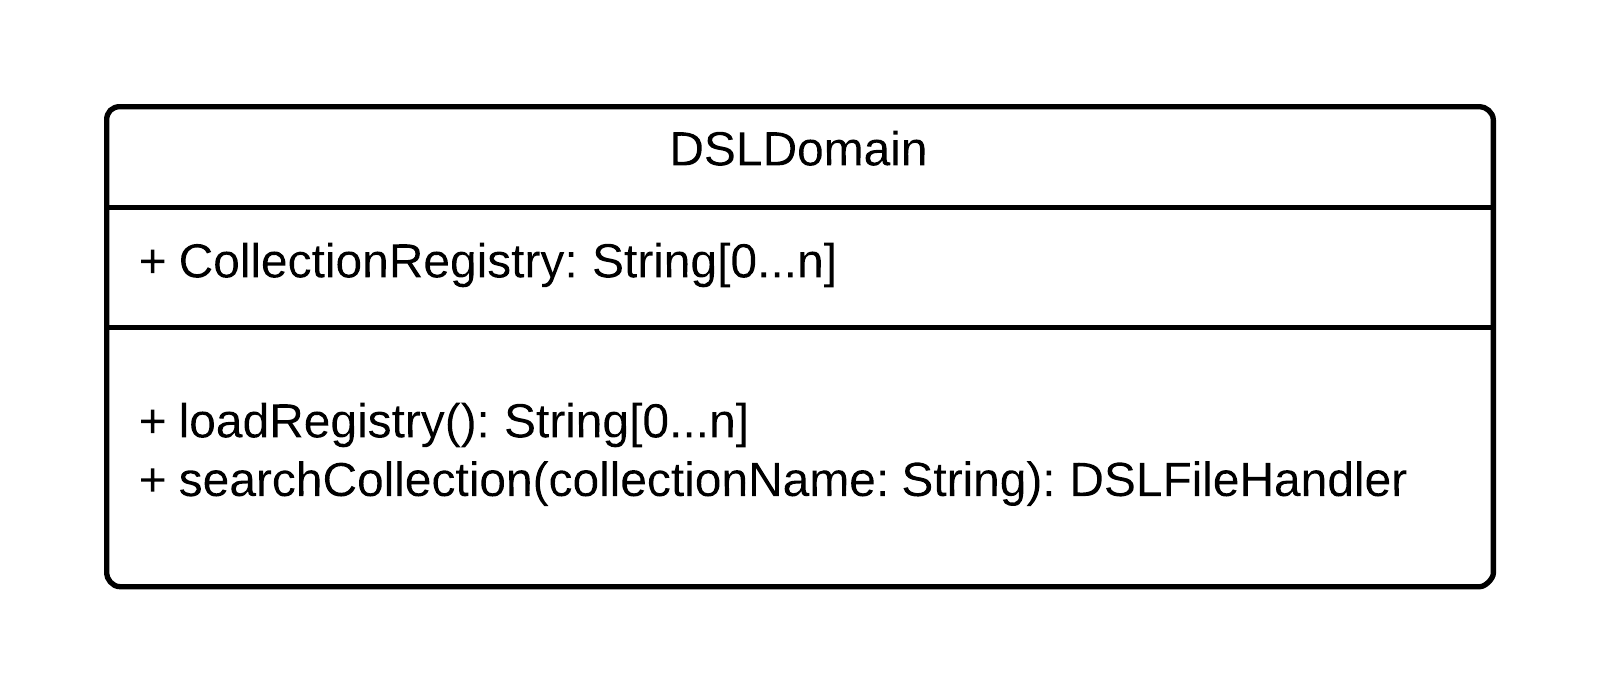
\includegraphics[width=0.6\textwidth]{patterns/contestualizzazione/registry.png}
\caption{Contestualizzazione di Registry}
\label{fig:mvc}
\end{figure}

\subsubsection{Factory method}

\begin{itemize}

	\item \textbf{Scopo}: Nel contesto di \glossario{Node.js} questo pattern viene usato creare una classe e restituire una sua istanza attraverso una \textit{funzione factory} che verrà esportata dal modulo. In questo modo si potrà costruire e ottenere qualsiasi classe definita in un modulo.
	\item \textbf{Utilizzo}: Alle basi del \textit{routing}, che utilizza la rappresentazione \glossario{REST}, vi sarà un controller associato per l'esecuzione delle diverse funzioni a seconda dell'URL indicato. In base a quest'ultimo dev'essere istanziata l'apposita classe che si occuperà di effettuare le sue funzioni. Per creare un oggetto di quella classe ci si avvale di una classe \textit{factory}, la quale si occuperà di invocare la costruzione dell'oggetto. Nell'architettura del progetto il pattern è implementato nella classe \texttt{Back-End::Lib::Controller::ControllerFactory}.

\end{itemize}

\begin{figure}[H]

\centering 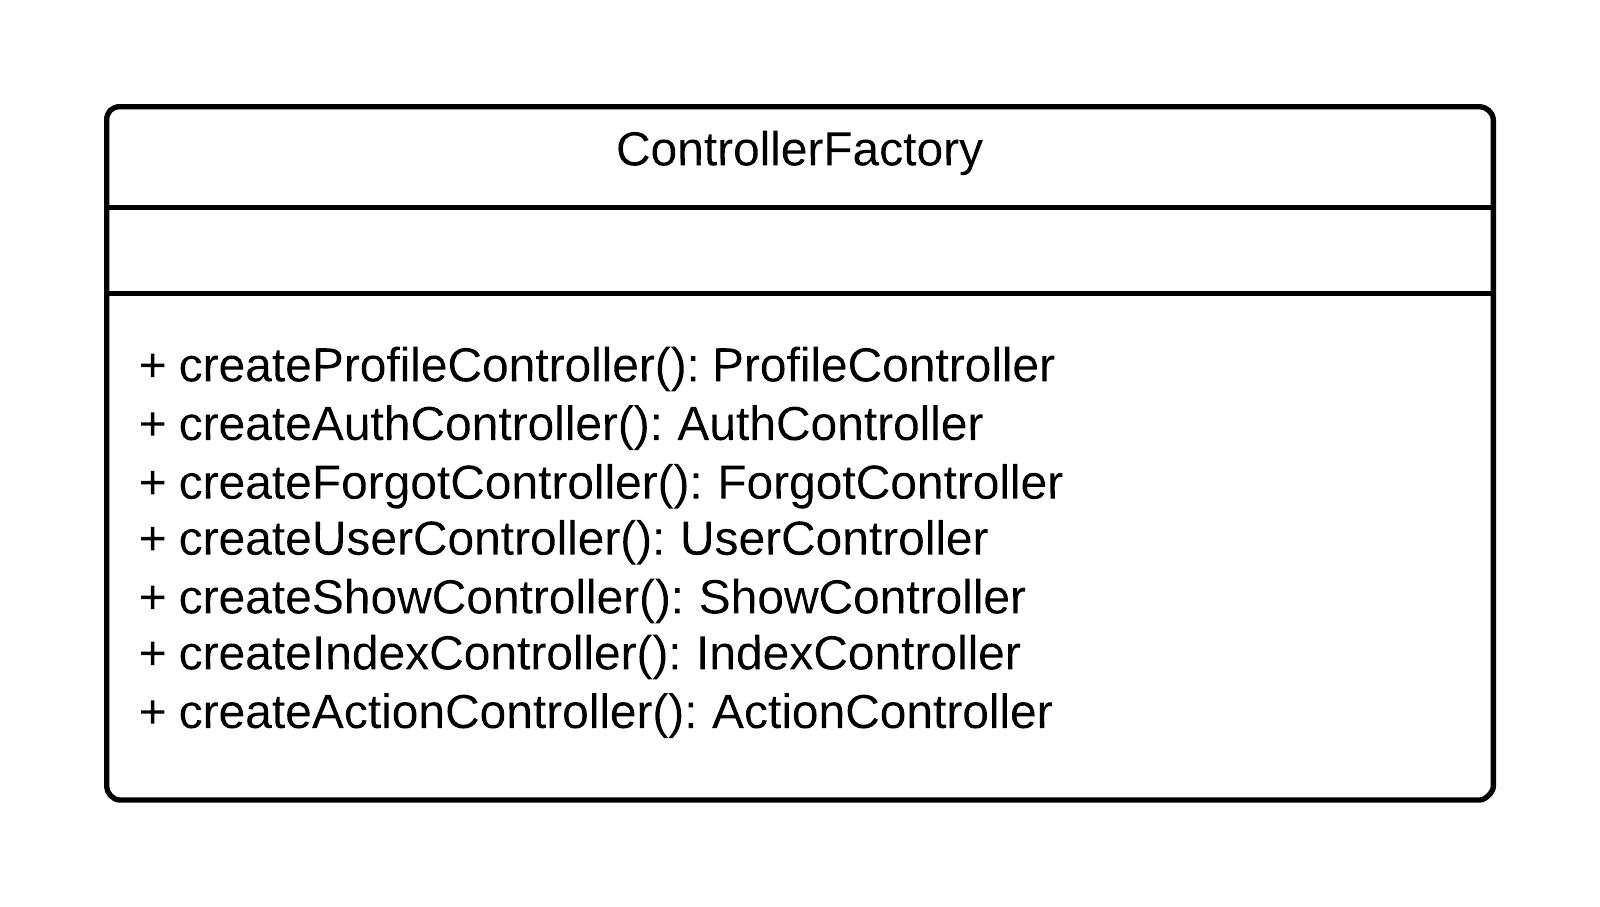
\includegraphics[width=0.6\textwidth]{patterns/contestualizzazione/factory-method.png}
\caption{Contestualizzazione di Factory Method}
\label{fig:mvc}
\end{figure}

\subsubsection{Singleton}

\begin{itemize}

	\item \textbf{Scopo}: Viene utilizzato per le classi che devono avere un'unica istanza durante l'esecuzione dell'applicazione;
	\item \textbf{Utilizzo}: Ogni modulo di \glossario{Node.js} è nativamente un singleton, perché viene caricato al primo \code{require} e poi tutti i successivi riferiscono allo stesso.

\end{itemize}

\subsection{Design Pattern Strutturali}

\subsubsection{Facade}

\begin{itemize}

	\item \textbf{Scopo}: Viene utilizzato per rendere visibili solamente alcune cose agli altri oggetti ed avere un unico punto di accesso semplificato a un sottosistema fornendo un'interfaccia di alto livello e minimizzando dunque le comunicazioni e le dipendenze.
	\item \textbf{Utilizzo}: Viene utilizzato all'interno della classe \\ \texttt{Back-End::Lib::Middleware::MiddlewareLoader}, la quale utilizza \textit{facade} per nascondere l'esistenza di tutti i \glossario{middleware} alla \texttt{ServerApp}. In questo modo le richieste vengono delegate agli oggetti appropriati senza che la classe cliente conosca le classi del sottosistema. Sarà il \textit{Facade} che si occuperà di trasferire la comunicazione all'oggetto appropriato.
\end{itemize}

\begin{figure}[H]

\centering 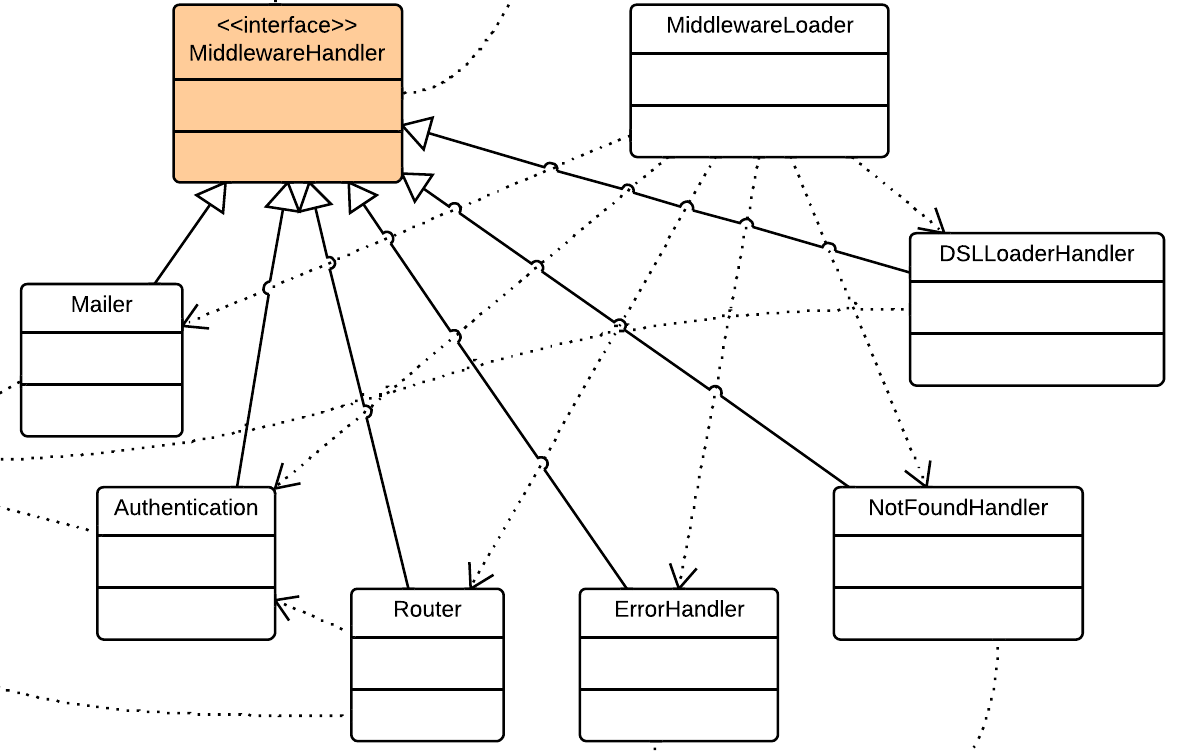
\includegraphics[width=0.6\textwidth]{patterns/contestualizzazione/facade1.png}
\caption{Contestualizzazione di Facade in \texttt{Back-End::Lib::Middleware::MiddlewareLoader}}
\label{fig:mvc}
\end{figure}

\subsection{Design Pattern Comportamentali}

\subsubsection{Chain of Responsibility}
\label{chain-of-responsibility}

\begin{itemize}

	\item \textbf{Scopo}: Viene utilizzato per far sì che un oggetto a cui viene effettuata una richiesta possa esaudire le richieste di più oggetti. In questo modo si evita l'accoppiamento fra il mittente di una richiesta e il destinatario. Tutti gli oggetti destinatari della richiesta sono \textit{concatenati} tra di loro. Ogni nodo della catena se può esaudire la richiesta la effettua, altrimenti delega l'onere al nodo successivo. La catena viene attraversata finché un nodo non può eseguire l'ordine del mittente. 
	\item \textbf{Utilizzo}: \glossario{Express} usa \textit{chain of Responsibility} per la gestione dei \glossario{middleware} e del \glossario{routing}. Come già accennato è particolarmente legato al pattern \textit{Middleware}. Viene utilizzato nella nostra architettura all'interno del package \texttt{Back-End::Lib::Middleware}. La classe \texttt{Back-End::Lib::Middleware::MiddlewareHandler} gestisce la richiesta scorrendo tutta la lista delle sottoclassi e richiamando il metodo \texttt{next} finché una di queste non può soddisfarla.

\end{itemize}

\begin{figure}[H]
\centering 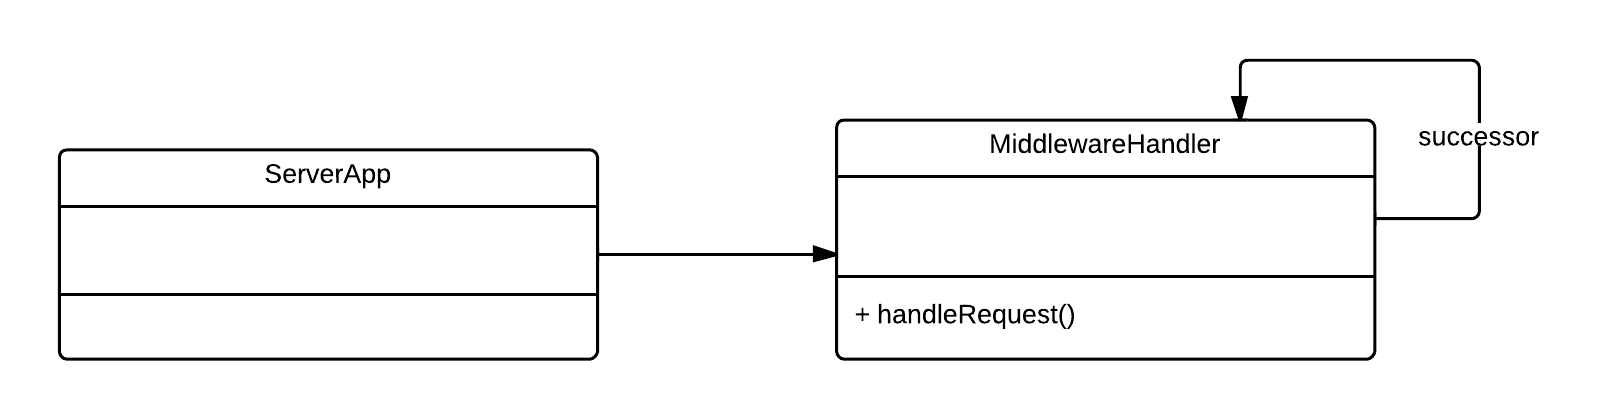
\includegraphics[width=0.6\textwidth]{patterns/contestualizzazione/chain-of-responsability.png}
\caption{Contestualizzazione di Chain of Responsibility}
\label{fig:mvc}
\end{figure}

\subsubsection{Strategy}

\begin{itemize}

	\item \textbf{Scopo}: Questo pattern serve per definire una famiglia di algoritmi e renderli intercambiabili, in modo che essi possano variare indipendentemente dal client che ne fa utilizzo. In un progetto software che guarda al futuro e che verrà manutenuto è fondamentale poter effettuare modifiche alle procedure in modo non intrusivo.
	\item \textbf{Utilizzo}: Viene utilizzato all'interno della classe \\ \texttt{Back-End::Lib::DSLModel::DSLInterpreterStrategy} in modo da permettere in futuro cambiamenti all'algoritmo di interpretazione del \glossario{DSL} senza dover intervenire sulla classe che ne fa uso, ovvero \texttt{Back-End::Lib::DSLModel::DSLDomain}.

\end{itemize}

\begin{figure}[H]
\centering 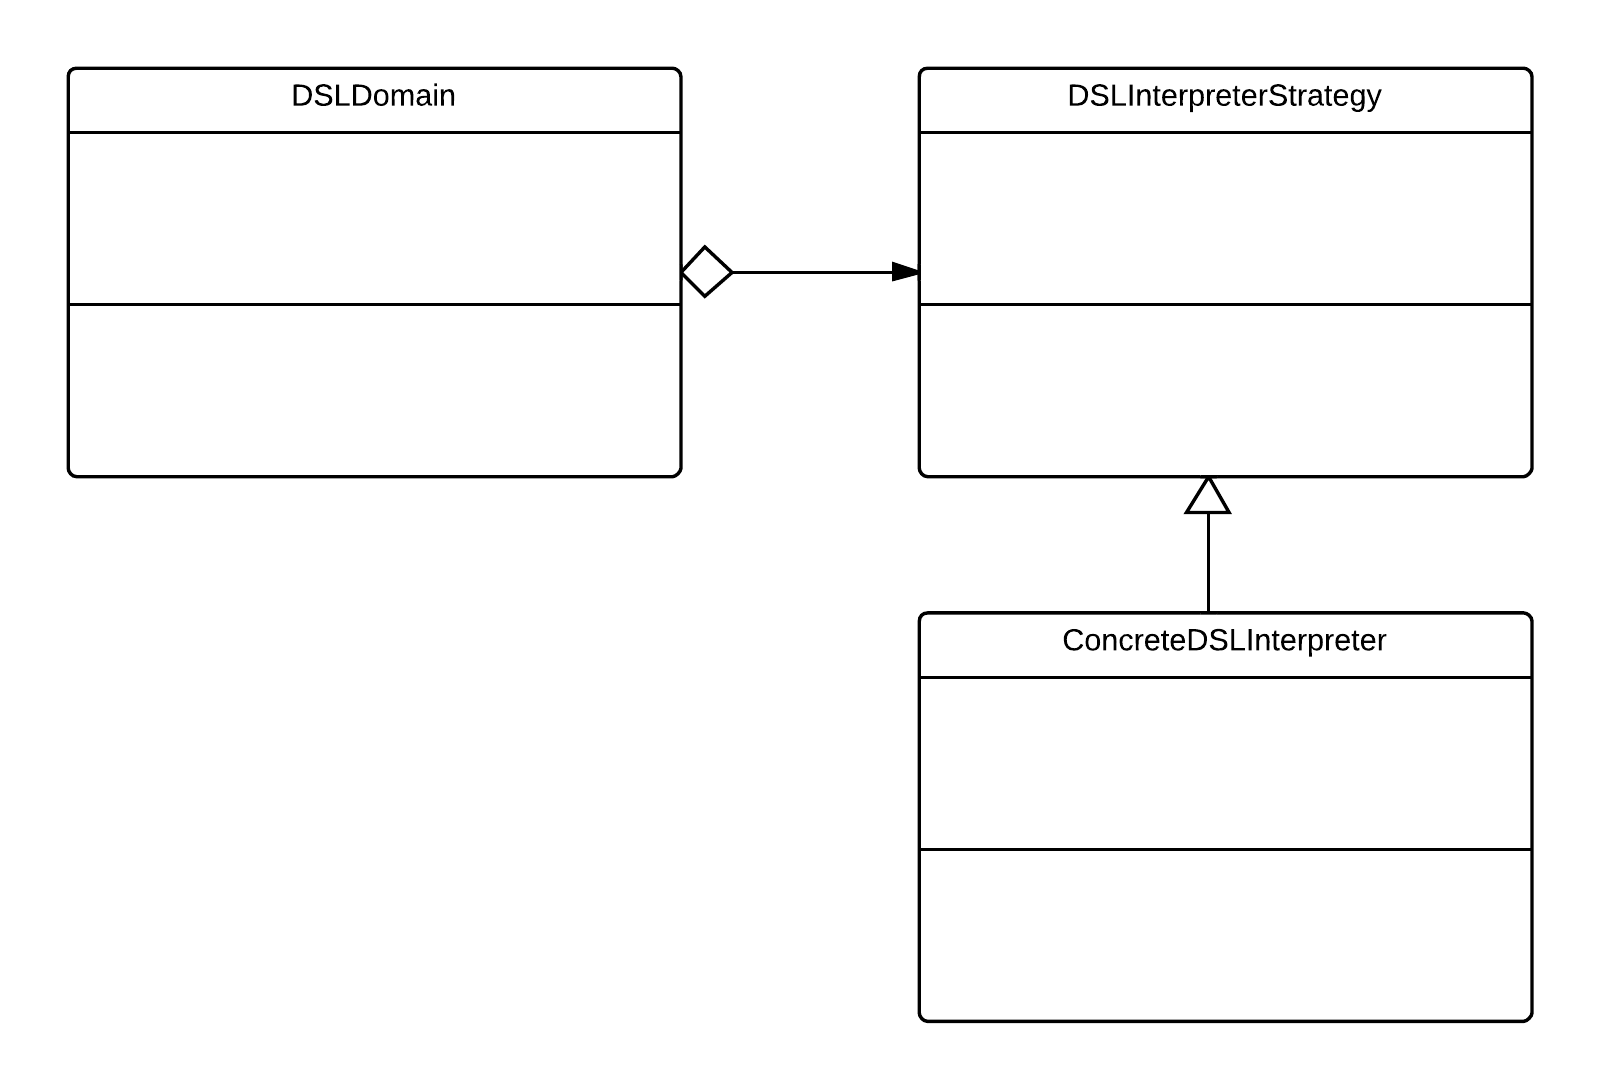
\includegraphics[width=0.6\textwidth]{patterns/contestualizzazione/strategy.png}
\caption{Contestualizzazione di Strategy}
\label{fig:mvc}
\end{figure}

\subsubsection{Command}

\begin{itemize}

	\item \textbf{Scopo}: Viene usato per parametrizzare gli oggetti rispetto a un'azione da compiere.
	\item \textbf{Utilizzo}: Viene utilizzato nel \glossario{package} \texttt{Back-End::DSLModel} per definire le azioni personalizzate da intraprendere sulle \glossario{Collection} o sui \glossario{Document}. In particolare \\ \texttt{Back-End::DSLModel::DocumentAction} e \texttt{Back-End::DSLModel::CollectionAction} rappresentano ciascuno il componente \textit{Command} del pattern (applicato in due contesti diversi). La componente \textit{ConcreteCommand} del pattern consiste in una delle due precedenti classi estese dinamicamente, ridefinendo un metodo.

\end{itemize}